\section{Grafici ed immagini}

\begin{figure}[h]
	\centering
	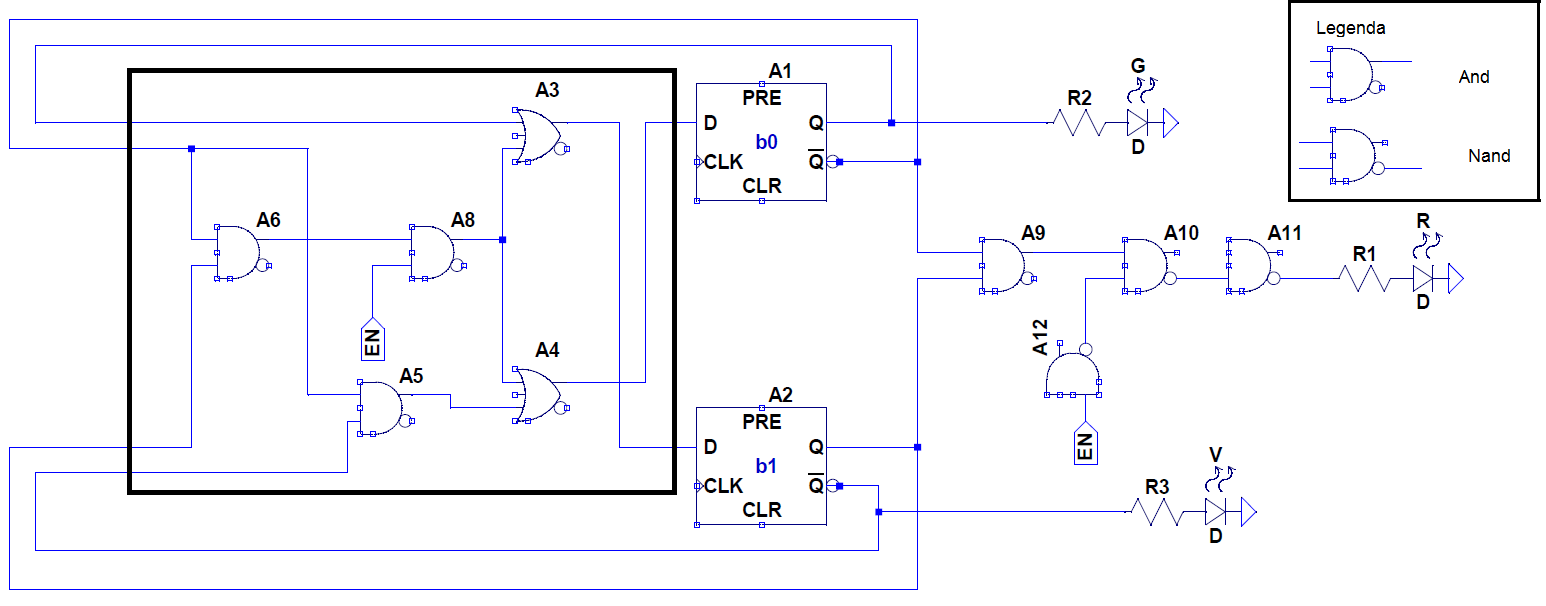
\includegraphics[scale=0.4]{circuito.png}
	\caption{Schema del circuito del semaforo completo.}
	\label{f:circuito_completo}
\end{figure}

\begin{figure}[h]
	\centering
	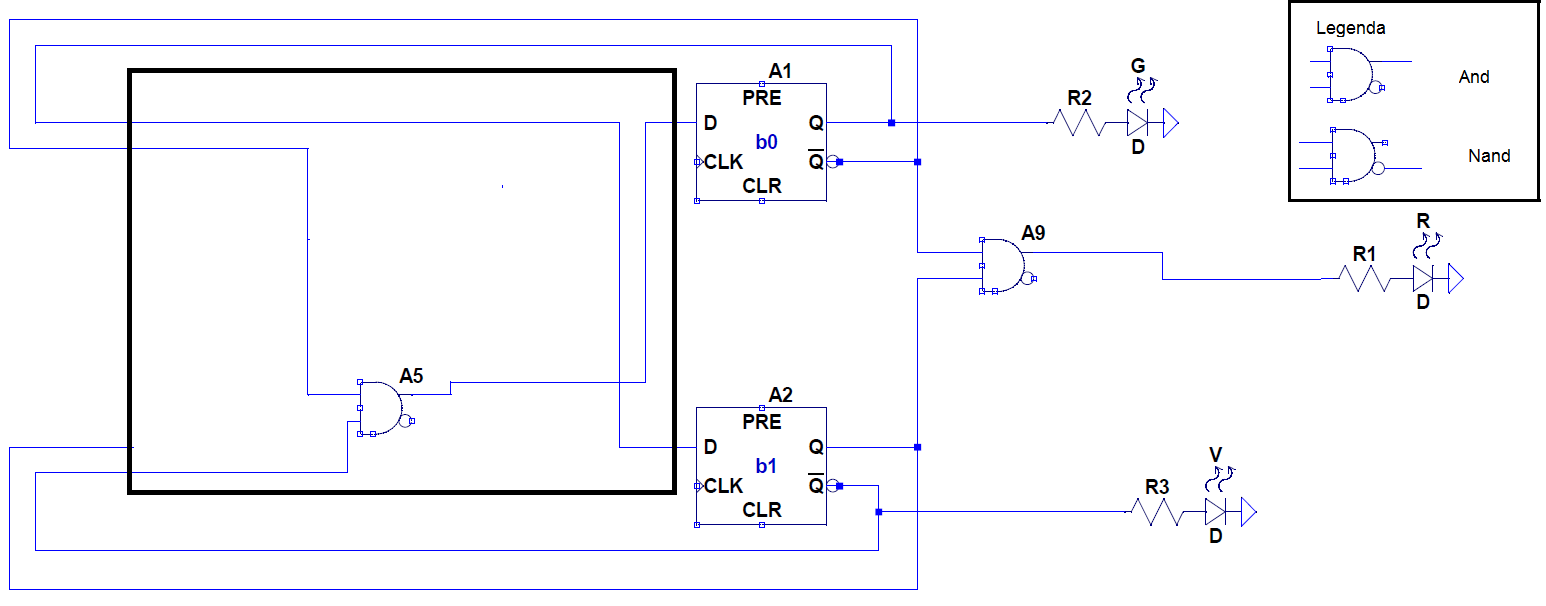
\includegraphics[scale=0.4]{circuito_abilitato.png}
	\caption{Schema del circuito del semaforo abilitato.}
	\label{f:semaforo_abilitato}
\end{figure}

\begin{figure}[h]
	\centering
	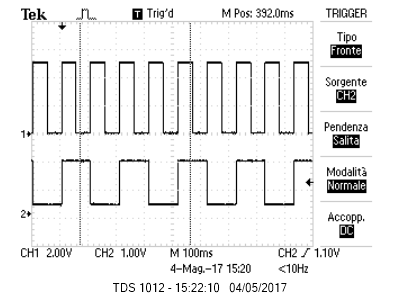
\includegraphics[scale=0.4]{clock-sopra--disabilitato-sotto.png}
	\caption{Il segnale in alto � il clock mentre quello in basso � il giallo lampeggiante.}
	\label{f:lampeggiante}
\end{figure}

\begin{figure}[h]
	\centering
	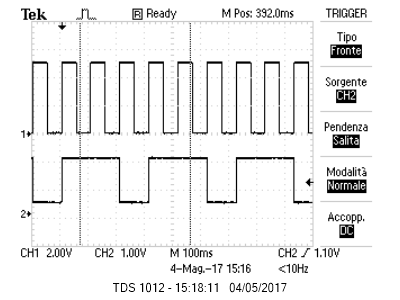
\includegraphics[scale=0.4]{clock-sopra--verde-sotto.png}
	\caption{Il segnale in alto � il clock mentre quello in basso � il verde nel caso di semaforo abilitato.}
	\label{f:verde}
\end{figure}

\begin{figure}[h]
	\centering
	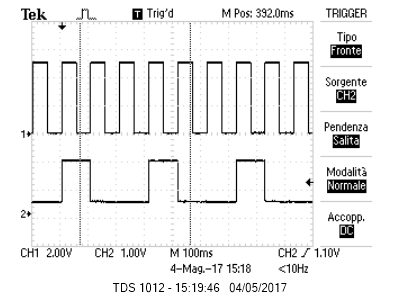
\includegraphics[scale=0.4]{clock-sopra--giallo-sotto.png}
	\caption{Il segnale in alto � il clock mentre quello in basso � il giallo nel caso di semaforo abilitato.}
	\label{f:giallo}
\end{figure}

\begin{figure}[h]
	\centering
	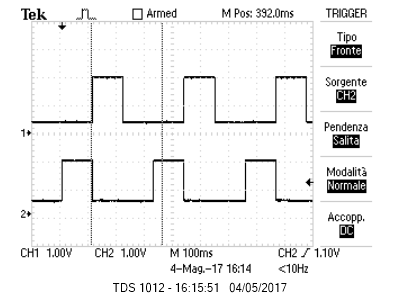
\includegraphics[scale=0.4]{rosso-sopra;giallo-sotto.png}
	\caption{Il segnale in alto � il rosso mentre quello in basso � il giallo,entrambi nel caso di semaforo abilitato.}
	\label{f:rosso}
\end{figure}

\begin{figure}[h]
	\centering
	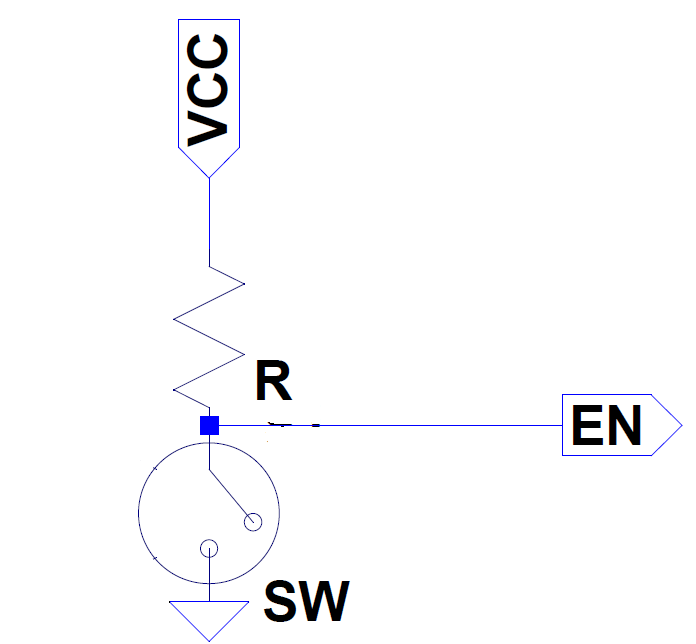
\includegraphics[scale=0.4]{switch.png}
	\caption{Schema circuitale usato per l'ENABLE.}
	\label{f:enable}
\end{figure}

\begin{figure}[h]
	\centering
	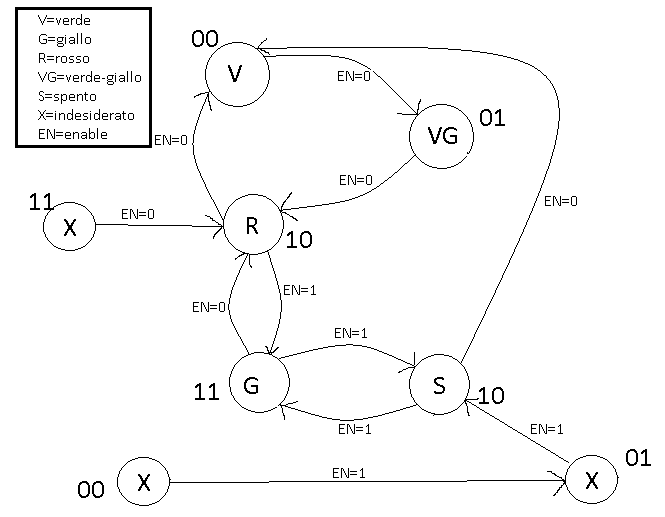
\includegraphics[scale=0.4]{diagramma di stato.png}
	\caption{Diagramma di stato per il semaforo completo.}
	\label{f:diagramma}
\end{figure}